\documentclass[11pt,a4paper]{report}
\usepackage[textwidth=37em,vmargin=30mm]{geometry}
\usepackage{calc,xunicode,amsmath,amssymb,paralist,enumitem,tabu,booktabs,datetime2,xeCJK,xeCJKfntef,listings}
\usepackage{tocloft,fancyhdr,tcolorbox,xcolor,graphicx,eso-pic,xltxtra,xelatexemoji}

\newcommand{\envyear}[0]{2024}
\newcommand{\envdatestr}[0]{2024-10-31}
\newcommand{\envfinaldir}[0]{webdb/2024/20241031/final}

\usepackage[hidelinks]{hyperref}
\hypersetup{
    colorlinks=false,
    pdfpagemode=FullScreen,
    pdftitle={Web Digest - \envdatestr}
}

\setlength{\cftbeforechapskip}{10pt}
\renewcommand{\cftchapfont}{\rmfamily\bfseries\large\raggedright}
\setlength{\cftbeforesecskip}{2pt}
\renewcommand{\cftsecfont}{\sffamily\small\raggedright}

\setdefaultleftmargin{2em}{2em}{1em}{1em}{1em}{1em}

\usepackage{xeCJK,xeCJKfntef}
\xeCJKsetup{PunctStyle=plain,RubberPunctSkip=false,CJKglue=\strut\hskip 0pt plus 0.1em minus 0.05em,CJKecglue=\strut\hskip 0.22em plus 0.2em}
\XeTeXlinebreaklocale "zh"
\XeTeXlinebreakskip = 0pt


\setmainfont{Brygada 1918}
\setromanfont{Brygada 1918}
\setsansfont{IBM Plex Sans}
\setmonofont{JetBrains Mono NL}
\setCJKmainfont{Noto Serif CJK SC}
\setCJKromanfont{Noto Serif CJK SC}
\setCJKsansfont{Noto Sans CJK SC}
\setCJKmonofont{Noto Sans CJK SC}

\setlength{\parindent}{0pt}
\setlength{\parskip}{8pt}
\linespread{1.15}

\lstset{
	basicstyle=\ttfamily\footnotesize,
	numbersep=5pt,
	backgroundcolor=\color{black!5},
	showspaces=false,
	showstringspaces=false,
	showtabs=false,
	tabsize=2,
	captionpos=b,
	breaklines=true,
	breakatwhitespace=true,
	breakautoindent=true,
	linewidth=\textwidth
}






\newcommand{\coverpic}[2]{
    % argv: itemurl, authorname
    Cover photo by #2~~(\href{#1}{#1})
}
\newcommand{\makeheader}[0]{
    \begin{titlepage}
        % \newgeometry{hmargin=15mm,tmargin=21mm,bmargin=12mm}
        \begin{center}
            
            \rmfamily\scshape
            \fontspec{BaskervilleF}
            \fontspec{Old Standard}
            \fontsize{59pt}{70pt}\selectfont
            WEB\hfill DIGEST
            
            \vfill
            % \vskip 30pt
            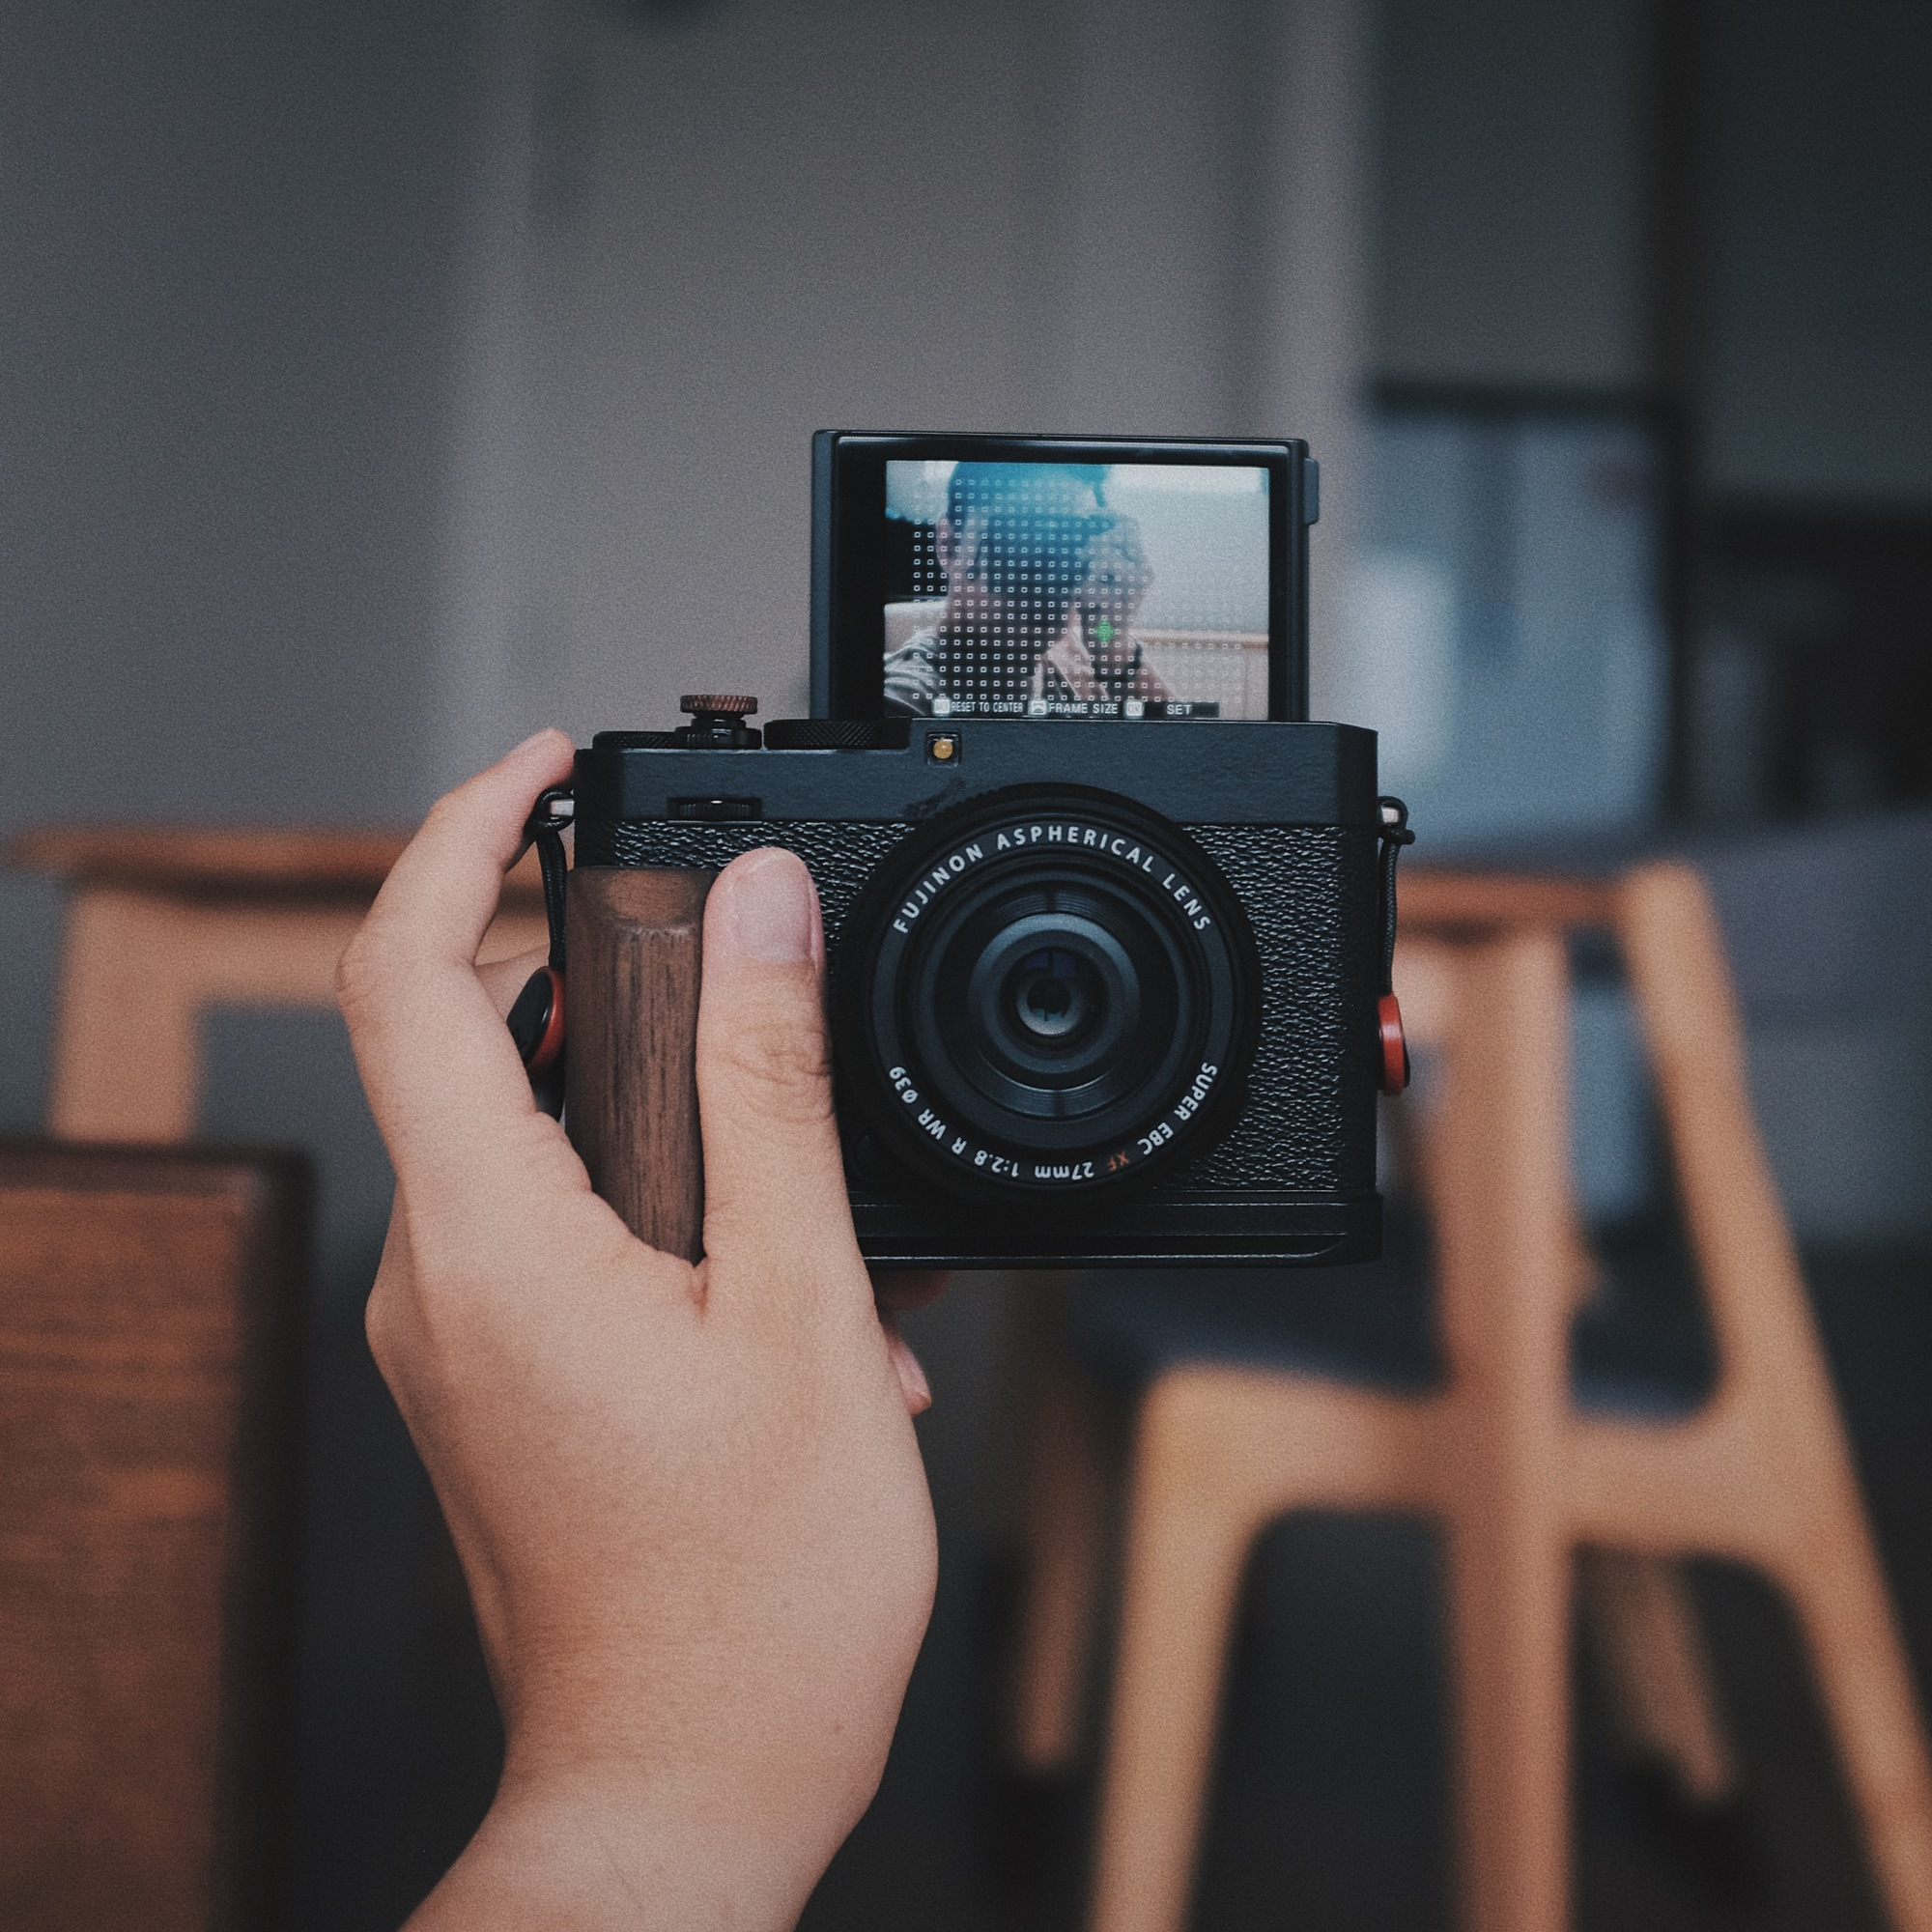
\includegraphics[width=\linewidth]{\envfinaldir/coverpic-prod.jpg}\par
            % \vskip 30pt
            \vfill

            \normalsize\rmfamily\scshape
            \copyright{} The Web Digest Project \hfill\large \envdatestr
        \end{center}
    \end{titlepage}
    % \restoregeometry
}
\newcommand{\simplehref}[1]{%
    \textcolor{blue!80!green}{\href{#1}{#1}}%
}
\renewcommand{\contentsname}{\center\Huge\sffamily\bfseries Contents\par\vskip 20pt}
\newcounter{ipartcounter}
\setcounter{ipartcounter}{0}
\newcommand{\ipart}[1]{
    % \vskip 20pt
    \clearpage
    \stepcounter{ipartcounter}
    \phantomsection
    \addcontentsline{toc}{chapter}{#1}
    % \begin{center}
    %     \Huge
    %     \sffamily\bfseries
    %     #1
    % \end{center}
    % \vskip 20pt plus 7pt
}
\newcounter{ichaptercounter}
\setcounter{ichaptercounter}{0}
\newcommand{\ichapter}[1]{
    % \vskip 20pt
    \clearpage
    \stepcounter{ichaptercounter}
    \phantomsection
    \addcontentsline{toc}{section}{\numberline{\arabic{ichaptercounter}}#1}
    \begin{center}
        \Huge
        \sffamily\bfseries
        #1
    \end{center}
    \vskip 20pt plus 7pt
}
\newcommand{\entrytitlefont}[1]{\subsection*{\raggedright\Large\sffamily\bfseries#1}}
\newcommand{\entryitemGeneric}[2]{
    % argv: title, url
    \parbox{\linewidth}{
        \entrytitlefont{#1}\par\vskip 5pt
        \footnotesize\ttfamily\mdseries
        \simplehref{#2}
    }\vskip 11pt plus 11pt minus 1pt
}
\newcommand{\entryitemGithub}[3]{
    % argv: title, url, desc
    \parbox{\linewidth}{
        \entrytitlefont{#1}\par\vskip 5pt
        \footnotesize\ttfamily\mdseries
        \simplehref{#2}\par\vskip 5pt
        \small\rmfamily\mdseries#3
    }\vskip 11pt plus 11pt minus 1pt
}
\newcommand{\entryitemAp}[3]{
    % argv: title, url, desc
    \parbox{\linewidth}{
        \entrytitlefont{#1}\par\vskip 5pt
        \footnotesize\ttfamily\mdseries
        \simplehref{#2}\par\vskip 5pt
        \small\rmfamily\mdseries#3
    }\vskip 11pt plus 11pt minus 1pt
}
\newcommand{\entryitemHackernews}[3]{
    % argv: title, hnurl, rawurl
    % \parbox{\linewidth}{
    %     \entrytitlefont{#1}\par\vskip 5pt
    %     \footnotesize\ttfamily\mdseries
    %     \simplehref{#3}\par
    %     \textcolor{black!50}{\href{#2}{#2}}
    % }\vskip 11pt plus 11pt minus 1pt
    \begin{minipage}{\linewidth}
            \entrytitlefont{#1}\par\vskip 5pt
            \footnotesize\ttfamily\mdseries
            \simplehref{#3}\par
            \textcolor{black!50}{\href{#2}{#2}}
    \end{minipage}\par\vskip 11pt plus 11pt minus 1pt
}







\begin{document}

\makeheader

\tableofcontents\clearpage




\ipart{Developers}
\ichapter{Hacker News}
\entryitemTwoLinks{Steam games will need to disclose kernel-level anti-cheat on store pages}{https://news.ycombinator.com/item?id=41999314}{https://www.gamingonlinux.com/2024/10/steam-games-will-now-need-to-fully-disclose-kernel-level-anti-cheat-on-store-pages/}

\entryitemTwoLinks{Google's TOS doesn't eliminate a user's Fourth Amendment rights, judge rules [pdf]}{https://news.ycombinator.com/item?id=41998891}{https://ww3.ca2.uscourts.gov/decisions/isysquery/0814a460-fe8f-42ef-9e82-cf94f952eb28/1/doc/23-6181\_opn.pdf}

\entryitemTwoLinks{BYD quarterly sales beat Tesla for first time}{https://news.ycombinator.com/item?id=41998840}{https://www.ft.com/content/fcc2db63-fb5a-4ae3-ab05-b8136b5193f4}

\entryitemTwoLinks{Cheap solar panels are changing the world}{https://news.ycombinator.com/item?id=41996425}{https://www.theatlantic.com/science/archive/2024/10/solar-power-energy-revolution-global-south/680351/}

\entryitemTwoLinks{M4 MacBook Pro}{https://news.ycombinator.com/item?id=41995701}{https://www.apple.com/newsroom/2024/10/new-macbook-pro-features-m4-family-of-chips-and-apple-intelligence/}

\entryitemTwoLinks{LLMs know more than they show: On the intrinsic representation of hallucinations}{https://news.ycombinator.com/item?id=41995201}{https://arxiv.org/abs/2410.02707}

\entryitemTwoLinks{Dropbox announces 20\% global workforce reduction}{https://news.ycombinator.com/item?id=41994640}{https://blog.dropbox.com/topics/company/an-update-from-drew}

\entryitemTwoLinks{Gross Apple Marketing}{https://news.ycombinator.com/item?id=41994567}{https://jonathanbuys.com/Gross\_Apple\_Marketing/}

\entryitemTwoLinks{EPA cancels pesticide shown to be harmful to unborn babies}{https://news.ycombinator.com/item?id=41993832}{https://www.thenewlede.org/2024/10/epa-cancels-pesticide-shown-to-be-harmful-to-unborn-babies/}

\entryitemTwoLinks{GLP-1s are among the most important drug breakthroughs}{https://news.ycombinator.com/item?id=41993782}{https://www.economist.com/briefing/2024/10/24/glp-1s-like-ozempic-are-among-the-most-important-drug-breakthroughs-ever}

\entryitemTwoLinks{Async Rust is not safe with io\_uring}{https://news.ycombinator.com/item?id=41992975}{https://tonbo.io/blog/async-rust-is-not-safe-with-io-uring}

\entryitemTwoLinks{Jaywalking legalized in New York City}{https://news.ycombinator.com/item?id=41992399}{https://www.theguardian.com/us-news/2024/oct/29/new-york-jaywalking-legal}

\entryitemTwoLinks{NASA reconnected with Voyager 1 after a brief pause}{https://news.ycombinator.com/item?id=41992394}{https://scitechdaily.com/15-billion-miles-away-nasas-voyager-1-breaks-its-silence/}

\entryitemTwoLinks{Australia/Lord\_Howe is the weirdest timezone}{https://news.ycombinator.com/item?id=41992314}{https://ssoready.com/blog/engineering/truths-programmers-timezones/}

\entryitemTwoLinks{Google CEO says more than a quarter of the company's new code is created by AI}{https://news.ycombinator.com/item?id=41991291}{https://www.businessinsider.com/google-earnings-q3-2024-new-code-created-by-ai-2024-10}

\entryitemTwoLinks{RIP botsin.space}{https://news.ycombinator.com/item?id=41989511}{https://muffinlabs.com/posts/2024/10/29/10-29-rip-botsin-space/}

\entryitemTwoLinks{GLP-1 for Everything}{https://news.ycombinator.com/item?id=41988285}{https://www.science.org/content/blog-post/glp-1-everything}

\entryitemTwoLinks{PhD student finds lost city in Mexico jungle}{https://news.ycombinator.com/item?id=41988171}{https://www.bbc.com/news/articles/crmznzkly3go}

\entryitemTwoLinks{OpenAI builds first chip with Broadcom and TSMC, scales back foundry ambition}{https://news.ycombinator.com/item?id=41986926}{https://www.reuters.com/technology/artificial-intelligence/openai-builds-first-chip-with-broadcom-tsmc-scales-back-foundry-ambition-2024-10-29/}

\entryitemTwoLinks{Using an 8K TV as a Monitor}{https://news.ycombinator.com/item?id=41986048}{https://daniel.lawrence.lu/blog/y2023m12d15/}\ichapter{Phoronix}
\entryitemGeneric{\hskip 0pt{}Ubuntu 25.04 "Plucky Puffin" Development Opens - Defaulting To -O3 Optimizations}{https://www.phoronix.com/news/Ubuntu-25.04-Plucky-Puffin}

\entryitemGeneric{\hskip 0pt{}Benchmarks Of Google's Axion Arm-based CPU: Competitive Performance \& Compelling Value}{https://www.phoronix.com/review/google-axion-c4a}

\entryitemGeneric{\hskip 0pt{}OpenPaX Announced As "Open-Source Alternative To GrSecurity" With Free Kernel Patch}{https://www.phoronix.com/news/Edera-OpenPaX-Announced}

\entryitemGeneric{\hskip 0pt{}DRM Panic "Screen of Death" Support Being Extended To All Recent AMD GPUs}{https://www.phoronix.com/news/AMD-DCE-DCN-DRM-Panic}

\entryitemGeneric{\hskip 0pt{}RadeonSI Lands Async Video Operations For Improving FFmpeg Performance}{https://www.phoronix.com/news/RadeonSI-Async-Video-Mesa}

\entryitemGeneric{\hskip 0pt{}VirtIO-GPU Vulkan Support Approaching Upstream QEMU}{https://www.phoronix.com/news/VirtIO-GPU-Vulkan-QEMU}

\entryitemGeneric{\hskip 0pt{}Wasmer 5.0 WebAssembly Runtime Released With V8, WAMR \& WASMI Backends}{https://www.phoronix.com/news/Wasmer-5.0-Released}

\entryitemGeneric{\hskip 0pt{}Shotcut 24.10 Open-Source Video Editor Adds Initial AI Feature}{https://www.phoronix.com/news/Shotcut-24.10-Released}

\entryitemGeneric{\hskip 0pt{}Intel Posts Updated Raptor Lake Microcode For Linux: Fixes Voltage Issue \& Other Bugs}{https://www.phoronix.com/news/Intel-RPL-Microcode-Voltage}\ichapter{Dribbble}
\entryitemGeneric{\hskip 0pt{}Lootbox}{https://dribbble.com/shots/24875582}

\entryitemGeneric{\hskip 0pt{}Internal Universe 🪐✨}{https://dribbble.com/shots/24870294}

\entryitemGeneric{\hskip 0pt{}Gulfstream x theory11 Playing Cards}{https://dribbble.com/shots/24869176}

\entryitemGeneric{\hskip 0pt{}Negative yet Positive Vol.7}{https://dribbble.com/shots/24868890}

\entryitemGeneric{\hskip 0pt{}Onton - Responsive Logo Design}{https://dribbble.com/shots/24866015}

\entryitemGeneric{\hskip 0pt{}Solufacil}{https://dribbble.com/shots/24869750}

\entryitemGeneric{\hskip 0pt{}Raw E}{https://dribbble.com/shots/24869489}

\entryitemGeneric{\hskip 0pt{}Ampersand 3D Logo}{https://dribbble.com/shots/24869500}

\entryitemGeneric{\hskip 0pt{}Rooster}{https://dribbble.com/shots/24854380}

\entryitemGeneric{\hskip 0pt{}cipher}{https://dribbble.com/shots/24855823}

\entryitemGeneric{\hskip 0pt{}"Amphiprion Ocellaris" - Daily art, NFT art}{https://dribbble.com/shots/24854577}

\entryitemGeneric{\hskip 0pt{}Bento Cards v.4 – E-Commerce}{https://dribbble.com/shots/24849627}

\entryitemGeneric{\hskip 0pt{}Neobanking Mobile App Interactions}{https://dribbble.com/shots/24848696}

\entryitemGeneric{\hskip 0pt{}FC Shakhtar Donetsk App. The Concept. Part 2}{https://dribbble.com/shots/24848383}

\entryitemGeneric{\hskip 0pt{}xflow Logo Design - X, Waves}{https://dribbble.com/shots/24847689}

\entryitemGeneric{\hskip 0pt{}The Future has landed ✈️}{https://dribbble.com/shots/24848230}

\entryitemGeneric{\hskip 0pt{}Converse Logo Redesign Concept}{https://dribbble.com/shots/24850036}

\entryitemGeneric{\hskip 0pt{}F Logo}{https://dribbble.com/shots/24850079}

\entryitemGeneric{\hskip 0pt{}ML Fashion 10/10}{https://dribbble.com/shots/24851262}

\entryitemGeneric{\hskip 0pt{}Amplemarket Logo Design}{https://dribbble.com/shots/24843224}

\entryitemGeneric{\hskip 0pt{}Streaming Data}{https://dribbble.com/shots/24838862}

\entryitemGeneric{\hskip 0pt{}It's not a feature, it's a bug}{https://dribbble.com/shots/24844082}

\entryitemGeneric{\hskip 0pt{}Cute Raccoon}{https://dribbble.com/shots/24843120}

\entryitemGeneric{\hskip 0pt{}Nero Code UI concept}{https://dribbble.com/shots/24843816}


\ipart{Developers~~~~(zh-Hans)}
\ichapter{Solidot}
\entryitemGeneric{\hskip 0pt{}苹果将 M4 Mac Mini 电源按钮移至底部}{https://www.solidot.org/story?sid=79636}

\entryitemGeneric{\hskip 0pt{}Dropbox 裁员五分之一}{https://www.solidot.org/story?sid=79635}

\entryitemGeneric{\hskip 0pt{}OpenAI 与博通和台积电合作设计 AI 芯片}{https://www.solidot.org/story?sid=79634}

\entryitemGeneric{\hskip 0pt{}X.Org Server 的一个本地提权漏洞存在了 18 年之久}{https://www.solidot.org/story?sid=79633}

\entryitemGeneric{\hskip 0pt{}索尼关闭《星鸣特攻》开发商 Firewalk Studio}{https://www.solidot.org/story?sid=79632}

\entryitemGeneric{\hskip 0pt{}中国三季度智能手机出货量增长 3.2\%}{https://www.solidot.org/story?sid=79631}

\entryitemGeneric{\hskip 0pt{}GitHub Copilot 将支持 Claude 3.5 和 Gemini 模型}{https://www.solidot.org/story?sid=79630}

\entryitemGeneric{\hskip 0pt{}Open Source Initiative 宣布 Open Source AI Definition 1.0}{https://www.solidot.org/story?sid=79629}

\entryitemGeneric{\hskip 0pt{}Fedora 41 释出}{https://www.solidot.org/story?sid=79628}

\entryitemGeneric{\hskip 0pt{}Firefox v132.0 释出}{https://www.solidot.org/story?sid=79627}

\entryitemGeneric{\hskip 0pt{}南非发现最古老的岩石微生物}{https://www.solidot.org/story?sid=79626}

\entryitemGeneric{\hskip 0pt{}Meta 开发 AI 搜索引擎}{https://www.solidot.org/story?sid=79625}

\entryitemGeneric{\hskip 0pt{}俄罗斯从马来西亚借道印度购买英伟达芯片}{https://www.solidot.org/story?sid=79624}

\entryitemGeneric{\hskip 0pt{}美国从明年 1 月起限制半导体和 AI 领域的对华投资}{https://www.solidot.org/story?sid=79623}

\entryitemGeneric{\hskip 0pt{}X 认证用户助长极化}{https://www.solidot.org/story?sid=79622}

\entryitemGeneric{\hskip 0pt{}苹果将教育游戏《俄勒冈小径》改编为电影}{https://www.solidot.org/story?sid=79621}

\entryitemGeneric{\hskip 0pt{}随着年龄增长鸟儿的朋友也会越来越少}{https://www.solidot.org/story?sid=79620}

\entryitemGeneric{\hskip 0pt{}Linus Torvalds 认为 AI 九成是营销一成才是现实}{https://www.solidot.org/story?sid=79619}

\entryitemGeneric{\hskip 0pt{}使用 AI 创建儿童色情的英国男子被判 18 年}{https://www.solidot.org/story?sid=79618}

\entryitemGeneric{\hskip 0pt{}联邦宇宙平台有了自己的短视频应用 Loops}{https://www.solidot.org/story?sid=79617}\ichapter{V2EX}
\entryitemGeneric{\hskip 0pt{}[程序员] AI 工具! 把笔记自动转换成 Anki 卡片}{https://www.v2ex.com/t/1085137}

\entryitemGeneric{\hskip 0pt{}[Apple] mbp m4 发布了,那么问题来了, 内存选 48G 还是 64G}{https://www.v2ex.com/t/1085136}

\entryitemGeneric{\hskip 0pt{}[Java] 请教后台接口如何根据前台的筛选条件动态构造查询 sql}{https://www.v2ex.com/t/1085135}

\entryitemGeneric{\hskip 0pt{}[Apple] 请教关于用 Mac mini 做外挂硬盘共享的问题}{https://www.v2ex.com/t/1085134}

\entryitemGeneric{\hskip 0pt{}[Apple] 有没有人研究下 Mac mini M4 + 外接屏幕替代 Mac book 的可行性?}{https://www.v2ex.com/t/1085133}

\entryitemGeneric{\hskip 0pt{}[小米] 小米手机如何卸载自带的讯飞,搜狗输入法?}{https://www.v2ex.com/t/1085132}

\entryitemGeneric{\hskip 0pt{}[汽车] 为什么某迪的车比不了小米??}{https://www.v2ex.com/t/1085131}

\entryitemGeneric{\hskip 0pt{}[macOS] 求推荐好看好用的第三方浏览器主页}{https://www.v2ex.com/t/1085130}

\entryitemGeneric{\hskip 0pt{}[macOS] 这个弹窗问题有解决方案吗}{https://www.v2ex.com/t/1085129}

\entryitemGeneric{\hskip 0pt{}[信息安全] 今天更新 Mull 被提示存在漏洞建议立即卸载}{https://www.v2ex.com/t/1085128}

\entryitemGeneric{\hskip 0pt{}[互联网] help:有全平台 read later 的 app 推荐么?}{https://www.v2ex.com/t/1085127}

\entryitemGeneric{\hskip 0pt{}[Apple] 请教下 Mac Mini 和 PC 共用一套有线鼠标键盘的方案?}{https://www.v2ex.com/t/1085126}

\entryitemGeneric{\hskip 0pt{}[问与答] 网易云的 NCM 格式是否更换了加密模式}{https://www.v2ex.com/t/1085124}

\entryitemGeneric{\hskip 0pt{}[Apple] macmini 外挂硬盘方案低成本 diy}{https://www.v2ex.com/t/1085122}

\entryitemGeneric{\hskip 0pt{}[macOS] 既然起步门槛升到 16G 了, 8G 用户是否应该留在 MacOs14?}{https://www.v2ex.com/t/1085121}

\entryitemGeneric{\hskip 0pt{}[问与答] 求助:通过代理回家成功,但连接 sunshine 远程桌面失败,如何排查解决}{https://www.v2ex.com/t/1085120}

\entryitemGeneric{\hskip 0pt{}[宽带症候群] 问下 J4125 和 N100 跑 ikuai 流控的性能}{https://www.v2ex.com/t/1085119}

\entryitemGeneric{\hskip 0pt{}[问与答] windows insider preview 上是不是只能安装 preview 版的 msoffice?}{https://www.v2ex.com/t/1085118}

\entryitemGeneric{\hskip 0pt{}[职场话题] 2 年 Java ,找工作好难,技术栈不对口完全没有机会}{https://www.v2ex.com/t/1085117}

\entryitemGeneric{\hskip 0pt{}[职场话题] 8 年 Java /Go 程序员,失业半年,未来何去何从}{https://www.v2ex.com/t/1085115}

\entryitemGeneric{\hskip 0pt{}[硬件] 各位大佬求推荐一款便宜的包月云电脑}{https://www.v2ex.com/t/1085114}

\entryitemGeneric{\hskip 0pt{}[投资] 2024.10.31 市场前瞻 写了下 AI 泡沫}{https://www.v2ex.com/t/1085112}

\entryitemGeneric{\hskip 0pt{}[前端开发] 有没有用 Lit 的朋友}{https://www.v2ex.com/t/1085111}

\entryitemGeneric{\hskip 0pt{}[信息安全] 为什么 VMP 壳没办法实现全自动脱壳,和它的哪些保护机制有关?}{https://www.v2ex.com/t/1085110}

\entryitemGeneric{\hskip 0pt{}[Kubernetes] containerd 使用镜像加速站的问题}{https://www.v2ex.com/t/1085109}

\entryitemGeneric{\hskip 0pt{}[程序员] [出海记录]开发新手的第 9 个站点上线}{https://www.v2ex.com/t/1085107}

\entryitemGeneric{\hskip 0pt{}[MacBook Pro] M4 可以选 32G 内存了,纠结中,求解惑}{https://www.v2ex.com/t/1085106}

\entryitemGeneric{\hskip 0pt{}[NAS] 求 DSM 转 TrueNAS Scale 建议}{https://www.v2ex.com/t/1085104}

\entryitemGeneric{\hskip 0pt{}[分享发现] [分享发现] 絵文字ミックス - 一个有趣的 Emoji 混合工具,支持 10 万种组合}{https://www.v2ex.com/t/1085103}

\entryitemGeneric{\hskip 0pt{}[Apple] iPhone16pro 港版是否支持 esim}{https://www.v2ex.com/t/1085102}

\entryitemGeneric{\hskip 0pt{}[Apple] 在售的 M2 和 M3 芯片版本 MacBook Air 标准版内存升级为 16GB,售价仍为 7999 元起。}{https://www.v2ex.com/t/1085101}

\entryitemGeneric{\hskip 0pt{}[奇思妙想] 有什么工具可以链接和整合各种知识库,并结合 AI 技术提高效率?}{https://www.v2ex.com/t/1085099}

\entryitemGeneric{\hskip 0pt{}[Apple] macbook air 应该明年春季不会有 m4 了,既然内存翻倍。}{https://www.v2ex.com/t/1085097}

\entryitemGeneric{\hskip 0pt{}[远程工作] [remote/头部交易所] 大数据测试工程师}{https://www.v2ex.com/t/1085094}

\entryitemGeneric{\hskip 0pt{}[macOS] iPhone 镜像输入法 bug,颜色显示不正常}{https://www.v2ex.com/t/1085093}

\entryitemGeneric{\hskip 0pt{}[智能家电] 海尔壁挂炉活动组队!}{https://www.v2ex.com/t/1085092}

\entryitemGeneric{\hskip 0pt{}[问与答] Macbook pro M4,这次苹果有挤牙膏吗?大家会买吗}{https://www.v2ex.com/t/1085091}

\entryitemGeneric{\hskip 0pt{}[音乐] 分享一个自建的工作 lofi 的 follow 列表,均为 lofi 视频,适合副屏播放,提升 coding 效率:)}{https://www.v2ex.com/t/1085090}

\entryitemGeneric{\hskip 0pt{}[Apple] Mac 热门系列更新完成, 连 M2 款 MacBook Air 都给了 16GB 内存, 价格不变}{https://www.v2ex.com/t/1085089}

\entryitemGeneric{\hskip 0pt{}[Linux] 有啥傻瓜式 docker compose up 就可以跑的旁路由透明网关吗?}{https://www.v2ex.com/t/1085088}

\entryitemGeneric{\hskip 0pt{}[Apple] 关于 mac mini 的性能有个问题}{https://www.v2ex.com/t/1085087}

\entryitemGeneric{\hskip 0pt{}[macOS] 有什么简单方案可以实现蓝牙连接后触发脚本吗?}{https://www.v2ex.com/t/1085086}

\entryitemGeneric{\hskip 0pt{}[Apple] MacBook Air 系列更新!加量不加价!标配 16G Ram}{https://www.v2ex.com/t/1085085}

\entryitemGeneric{\hskip 0pt{}[Apple] M4 MacBook Pro 发布}{https://www.v2ex.com/t/1085084}

\entryitemGeneric{\hskip 0pt{}[Apple] MacBook Pro M4 系列发布了,三天的产品发布完成}{https://www.v2ex.com/t/1085083}

\entryitemGeneric{\hskip 0pt{}[问与答] 大家的 mac 键盘都改键位吗}{https://www.v2ex.com/t/1085082}

\entryitemGeneric{\hskip 0pt{}[MacBook Pro] M4 Pro/Max 的 MacBook Pro 发布了,没有 Studio。 M4 Max 较上代提升 20\%}{https://www.v2ex.com/t/1085080}

\entryitemGeneric{\hskip 0pt{}[职场话题] 沉浮土木路}{https://www.v2ex.com/t/1085079}

\entryitemGeneric{\hskip 0pt{}[远程工作] [remote/头部交易所] 业务后台产品经理}{https://www.v2ex.com/t/1085078}

\entryitemGeneric{\hskip 0pt{}[酷工作] IT 系统工程师,地点:上海,薪资: 20-35k,年龄 30 以内, 985 院校}{https://www.v2ex.com/t/1085077}


\ipart{Generic News}
\ichapter{AP News}
\entryitemWithDescription{\hskip 0pt{}A New Zealand city waves goodbye to its giant hand sculpture that many came to love}{https://apnews.com/article/cfcd3599eda341b78741dcfcf519edbd}{}

\entryitemWithDescription{\hskip 0pt{}Yankees beat Dodgers to force World Series Game 5}{https://apnews.com/article/1ae2f34295846e1df14b0f7fdb33b0b2}{}

\entryitemWithDescription{\hskip 0pt{}Democrats are leaning on celebrity star power. Will it matter?}{https://apnews.com/article/5974cc15b79220bd0b5a0bf561c21c23}{}

\entryitemWithDescription{\hskip 0pt{}Teri Garr, the offbeat comic actor of `Young Frankenstein' and `Tootsie,' has died}{https://apnews.com/article/be39482a60724c5bb81bbd8f34dfaf2d}{}

\entryitemWithDescription{\hskip 0pt{}In a first since 1938, Des Moines, Iowa, kids will trick-or-treat on Halloween}{https://apnews.com/article/26710c8e3564d461b6868313f7f71425}{}

\entryitemWithDescription{\hskip 0pt{}Teen fights kidney failure after eating McDonald's Quarter Pounders}{https://apnews.com/article/acb6d87f6182b42295d16625480525b0}{}

\entryitemWithDescription{\hskip 0pt{}A second high court rules that Japan's ban on same-sex marriage is unconstitutional}{https://apnews.com/article/6005ae890fdc7fd176ce72b57a1f7d99}{}

\entryitemWithDescription{\hskip 0pt{}Pro Women's Hockey League says it could add as many as two teams for 2025-26 season}{https://apnews.com/article/20e84fec388fd3b29a0c54ee0c5c7a33}{}

\entryitemWithDescription{\hskip 0pt{}Rapper Tekashi 6ix9ine is detained in New York on parole violation claims}{https://apnews.com/article/fce37fb6764c70a0ee194f25f318c8bc}{}

\entryitemWithDescription{\hskip 0pt{}CNN bans conservative panelist after on-air remark to Muslim commentator}{https://apnews.com/article/713c5c8c2f4c8b221b8d83fc20597308}{}

\entryitemWithDescription{\hskip 0pt{}Man standing trial alongside rapper Young Thug accepts plea deal}{https://apnews.com/article/a9859b163d2711254b86479a1f3e9d6a}{}

\entryitemWithDescription{\hskip 0pt{}UFC champ Jon Jones agrees to anger management classes to resolve assault charge}{https://apnews.com/article/f8959f5b469169bef5d4f2076caba97b}{}

\entryitemWithDescription{\hskip 0pt{}A tram derails and plows into a shop in the Norwegian capital but only 4 are lightly injured}{https://apnews.com/article/666020291c635d8b1f99330a971c2618}{}\ichapter{Reuters}
\entryitemWithDescription{\hskip 0pt{}Mexico's lower house votes to ban challenges to constitutional reforms}{https://www.reuters.com/world/americas/mexicos-lower-house-votes-ban-challenges-constitutional-reforms-2024-10-30/}{Mexico\textquotesingle s lower house of Congress approved a constitutional reform on Wednesday that makes reforms to the constitution "unchallengeable" as ruling party Morena and allies push through a swath of constitutional reforms...}

\entryitemWithDescription{\hskip 0pt{}Taiwan shuts down for arrival of Super Typhoon Kong-rey}{https://www.reuters.com/world/asia-pacific/taiwan-shuts-down-arrival-super-typhoon-kong-rey-2024-10-30/}{Taiwan shut down ahead of the arrival of Super Typhoon Kong-rey on Thursday with all cities and counties declaring a day off, financial markets closed and domestic flights cancelled for what is expected to be the largest storm by size in...}

\entryitemWithDescription{\hskip 0pt{}Bolivia president calls for end of blockades, says costs pass \$1.7 billion}{https://www.reuters.com/world/americas/bolivia-has-lost-over-17-billion-due-blockades-says-president-2024-10-30/}{Bolivian president on Wednesday called for the end of costly highway blockades that have paralyzed parts of the country and fueled an increasingly volatile conflict with his main political...}

\entryitemWithDescription{\hskip 0pt{}Australia must brace for longer fire seasons and marine heatwaves ahead, report says}{https://www.reuters.com/world/asia-pacific/australia-must-brace-longer-fire-seasons-marine-heatwaves-ahead-report-says-2024-10-30/}{Australia must brace for longer and more dangerous fire seasons and marine heatwaves in the years ahead, while swift changes in weather patterns might result in more hot days and fewer cool days, a government report said on...}

\entryitemWithDescription{\hskip 0pt{}North Korea fires long-range ballistic missile, South Korea says}{https://www.reuters.com/world/asia-pacific/north-korea-fires-ballistic-missile-yonhap-2024-10-30/}{North Korea fired a suspected long-range ballistic missile towards the sea off its east coast on Thursday, South Korea\textquotesingle s Joint Chiefs of Staff said, a day after Seoul reported the North was making preparations to test...}

\entryitemWithDescription{\hskip 0pt{}Russian bomb hits residential building in Ukraine's Kharkiv, 17 injured, major damage}{https://www.reuters.com/world/europe/russian-bomb-hits-residential-building-ukraines-kharkiv-there-are-casualties-2024-10-30/}{A Russian guided bomb struck a high-rise apartment block on Wednesday evening in Kharkiv, Ukraine\textquotesingle s second largest city, injuring at least 17 people, including three trapped under rubble, and badly damaging the building...}

\entryitemWithDescription{\hskip 0pt{}French PhD student detained in Tunisia on breach of state security charges, lab director says}{https://www.reuters.com/world/french-phd-student-detained-tunisia-breach-state-security-charges-lab-director-2024-10-30/}{French PhD student Victor Dupont was detained in Tunisia on breach of state security charges 12 days ago, and French authorities are trying to negotiate his release, the director of his research lab, Vincent Geisser...}

\entryitemWithDescription{\hskip 0pt{}IMF board approves Kenya's reviews, unlocking access to \$606 million}{https://www.reuters.com/world/africa/imf-board-approves-kenyas-reviews-unlocking-access-606-million-2024-10-30/}{The executive board of the International Monetary Fund has approved the seventh and eighth reviews of Kenya\textquotesingle s program, the IMF said on Wednesday, paving the way for the cash-strapped government to access a \$606 million...}

\entryitemWithDescription{\hskip 0pt{}Israeli strikes kill 19 people including eight women in two towns in Lebanon's Baalbek, health ministry says}{https://www.reuters.com/world/middle-east/israeli-strikes-kill-19-people-including-eight-women-two-towns-lebanons-baalbek-2024-10-30/}{Israeli strikes killed 19 people including eight women in two towns in Lebanon\textquotesingle s Baalbek region, the Lebanese health ministry said on...}

\entryitemWithDescription{\hskip 0pt{}Argentine President Milei fires foreign minister after vote to lift embargo against Cuba}{https://www.reuters.com/world/americas/argentinas-milei-fires-foreign-minister-after-vote-lift-embargo-against-cuba-2024-10-30/}{Argentina\textquotesingle s President Javier Milei on Wednesday replaced Foreign Affairs Minister Diana Mondino after she voted in favor of lifting the U.S. embargo against Cuba at the United...}

\entryitemWithDescription{\hskip 0pt{}Russia asks at UN: If West aids Ukraine, why can't North Korea help us?}{https://www.reuters.com/world/russia-tells-un-cooperation-with-north-korea-does-not-violate-international-law-2024-10-30/}{Russia\textquotesingle s envoy to the United Nations on Wednesday questioned why its allies like North Korea could not help Moscow in its war against Ukraine given Western countries claim the right to help...}

\entryitemWithDescription{\hskip 0pt{}UN urges probe of killings in Bangladesh protests, minority protection}{https://www.reuters.com/world/asia-pacific/un-urges-probe-killings-bangladesh-protests-minority-protection-2024-10-30/}{A top UN official on Wednesday urged a probe into the killings in Bangladesh during protests that led to the downfall of ousted Prime Minister Sheikh Hasina, while also calling for minority protection and a national process of truth and...}

\entryitemWithDescription{\hskip 0pt{}Biden will attend US presidential inauguration regardless of winner, White House says}{https://www.reuters.com/world/us/biden-will-attend-us-presidential-inauguration-regardless-winner-white-house-2024-10-30/}{President Joe Biden will attend the inauguration of the next U.S. president in January regardless of who wins next Tuesday\textquotesingle s election, White House spokesperson Karine Jean-Pierre told reporters on Wednesday, vowing a...}






\clearpage
\leavevmode\vfill
\footnotesize

Copyright \copyright{} 2023-2024 Neruthes and other contributors.

This document is published with CC BY-NC-ND 4.0 license.

The entries listed in this newsletter may be copyrighted by their respective creators.

This newsletter is generated by the Web Digest project.

The newsletters are also delivered via Telegram channel \CJKunderline{\href{https://t.me/webdigestchannel}{https://t.me/webdigestchannel}}.\\
RSS feed is available at \CJKunderline{\href{https://webdigest.pages.dev/rss.xml}{https://webdigest.pages.dev/rss.xml}}.

This newsletter is available in PDF at
\CJKunderline{\href{https://webdigest.pages.dev/}{https://webdigest.pages.dev/}}.

The source code being used to generate this newsletter is available at\\
\CJKunderline{\href{https://github.com/neruthes/webdigest}{https://github.com/neruthes/webdigest}}.

This newsletter is also available in
\CJKunderline{\href{http://webdigest.pages.dev/readhtml/\envyear/WebDigest-20241031.html}{HTML}} and
\CJKunderline{\href{https://github.com/neruthes/webdigest/blob/master/markdown/\envyear/WebDigest-20241031.md}{Markdown}}.


\coverpic{https://unsplash.com/photos/a-mountain-is-silhouetted-against-an-orange-sky-dgFA4gswn\_4}{Maksim Samuilionak}


\end{document}
